\section{Question 3}

\subsection{The Question}



 Consider the "bow-tie" graph in the Broder et al. paper (fig 9):
    \url{http://www9.org/w9cdrom/160/160.html}

    Now consider the following graph:

\begin{multicols}{4}


    A $ \rightarrow $ B

    B $ \rightarrow $ C

    C $ \rightarrow $  D

    C $ \rightarrow $ A

\columnbreak

    C $ \rightarrow $  G

    E  $ \rightarrow $  F

    G $ \rightarrow $ C

    G $ \rightarrow $ H

    I $ \rightarrow $ H

\columnbreak

    I $ \rightarrow $ J

    I $ \rightarrow $ K

    J $ \rightarrow $ D 

    L $ \rightarrow $ D

\columnbreak

    M $ \rightarrow $ A

    M $ \rightarrow $ N

    N $ \rightarrow $ D
    
\end{multicols}




    For the above graph, give the values for:  IN,   SCC,    OUT,  Tendrils,     Tubes,     Disconnected

\subsection{The Answer}


The most critical part of analyzing a graph and identifying the constituent components is to find the strongly connected component. This can be done visually or heuristically in this case. However, in the case of complex and large networks this is not an efficient method. Thankfully algorithms have been developed to solve this problem and they are implemented in python libraries. This way we can verify the result we obtain manually. 




\begin{figure}
\centering
	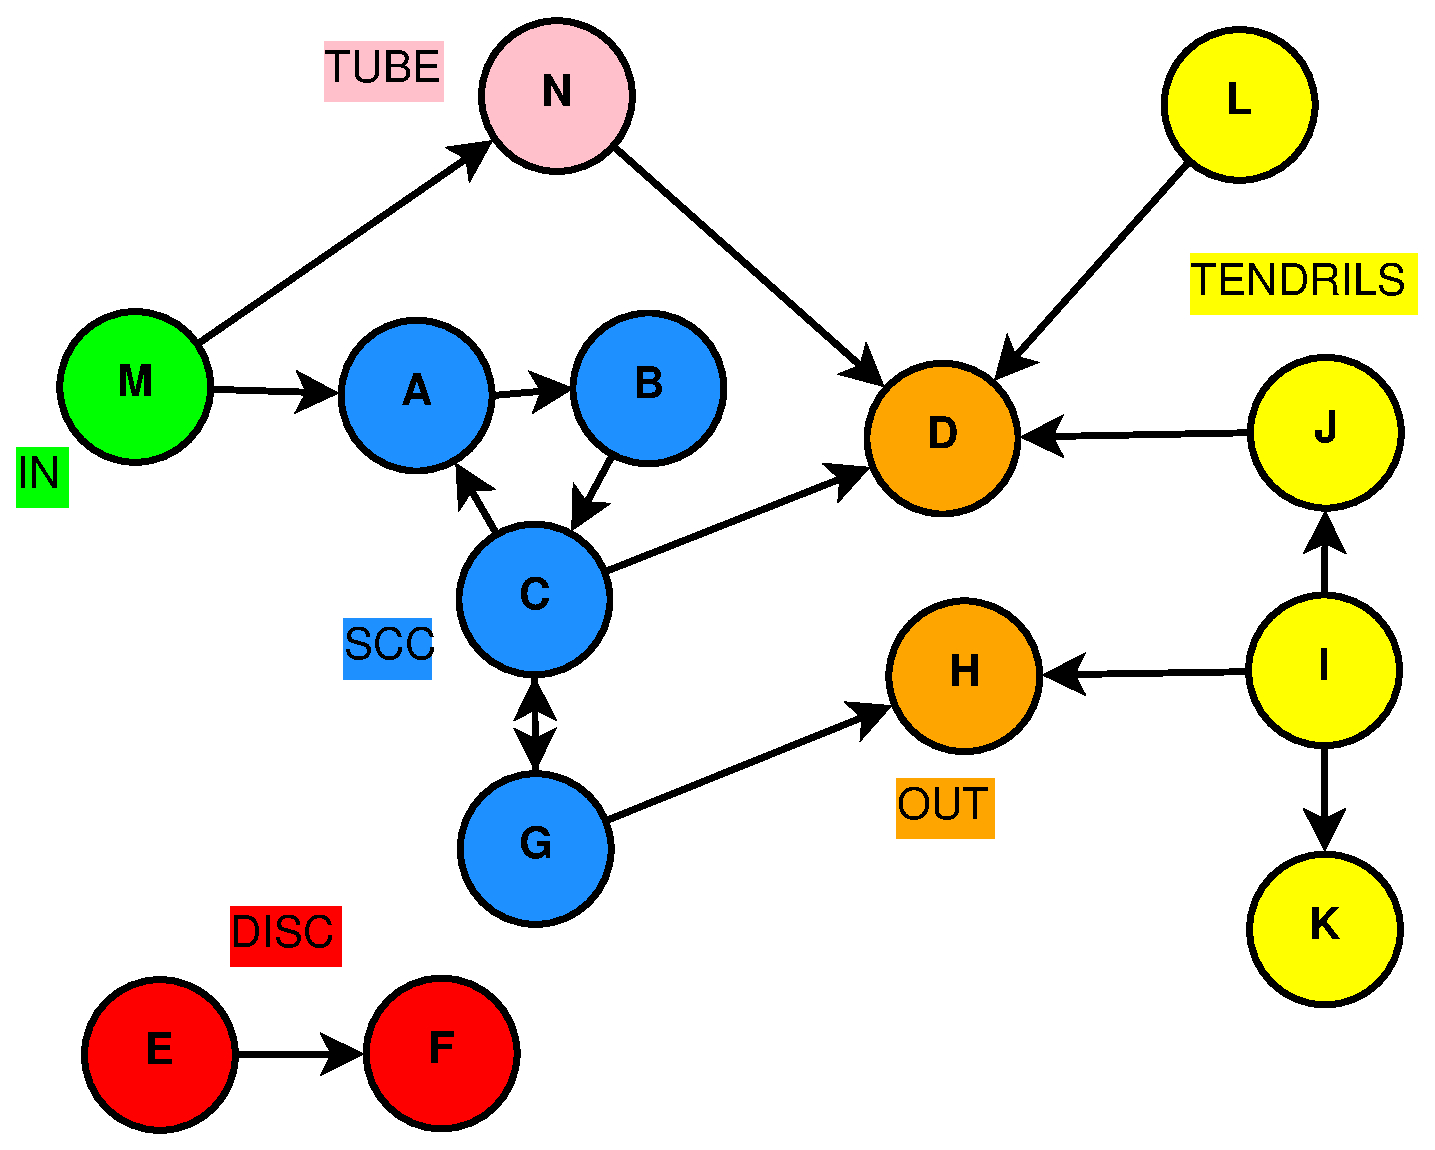
\includegraphics[width=.8\textwidth]{figures/graphLabel.eps}
	
\end{figure}


\pagebreak

\lstset{
    language=python,
    label=code:correction_8.5,
    caption={Code Listing the relevance file corrector}
}

\lstinputlisting{../q3/graphSc.py}